\documentclass[10pt]{article}
\usepackage[utf8]{inputenc}
\usepackage[final]{graphics}
\usepackage[pdftex]{graphicx}
\usepackage[dvips]{color}
\usepackage{amsfonts}
\usepackage{subfigure}
\usepackage{lscape}
\usepackage{hyperref}
\usepackage{amsmath}
\usepackage{units}
\usepackage{float}
\usepackage[table]{xcolor}
\usepackage[magyar]{babel}
\addtolength{\oddsidemargin}{-3.5cm}
\addtolength{\textwidth}{7cm}
\addtolength{\topmargin}{-3cm}
\addtolength{\textheight}{5cm}
\newcommand{\hide}[1]{}
\DeclareGraphicsExtensions{.jpg,.pdf,.mps,.png}
\usepackage{tikz}
\usetikzlibrary{scopes}

\title{Forgómozgás vizsgálata}
\author{Mérést végezte: Kalló Bernát $\diamondsuit$ Mérőtárs: Magony Miklós}
\date{Mérés dátuma: 2012. 03. 28. Leadás dátuma: 2012. 04. 11.}
\begin{document}
\maketitle

\def\Ms{\ensuremath{M_s}}\def\rho{\ensuremath{\varrho}}\def\Thetamert{\ensuremath{\Theta_{\text{mért}}}}\def\Thetaszam{\ensuremath{\Theta_{\text{szám}}}}\def\DeltaThetamert{\ensuremath{\Delta\ensuremath{\Theta_{\text{mért}}}}}\def\DeltaThetaszam{\ensuremath{\Delta\ensuremath{\Theta_{\text{szám}}}}}\def\deltaThetamert{\ensuremath{\delta\ensuremath{\Theta_{\text{mért}}}}}\def\deltaThetaszam{\ensuremath{\delta\ensuremath{\Theta_{\text{szám}}}}}\def\korong{\text{korong}}\def\rud{\text{rúd}}\def\fonal{\text{fonaltárcsa}}\def\Thetarud{\ensuremath{\ensuremath{\Theta} _{\text{rúd}}}}\def\Thetakorong{\ensuremath{\ensuremath{\Theta}_{\text{korong}}}}\def\mfonal{\ensuremath{m_{\text{fonaltárcsa}}}}


\paragraph*{A mérés célja}
Két, rögzített tengely körül forgó merev test (egy függőleges tengelyű alumínium korong és egy vízszintes tengelyű rézhenger) mozgását vizsgáljuk külső forgatónyomaték hatására. Megmérjük a szöggyorsulását, ebből kiszámoljuk tehetetlenségi nyomatékukat, és összevetjük a geometriájuk alapján számítottal.

\paragraph*{A mérés leírása}
A függőleges tengely körül szabadon forgó próbatestet egy orsóra tekert fonálon keresztül egy csigán lelógó súly húzza.
Két különböző próbatestet vizsgálunk 6-6 különböző húzósúllyal, és megmérjük a kötél gyorsulását.

\begin{figure}[H]
\begin{center}
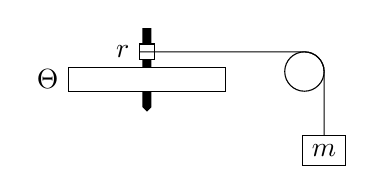
\begin{tikzpicture}

\draw[fill=black] (-.05,1) -- (-.05,0) -- (0,-.05) -- (.05,0) -- (.05,1);
\draw[fill=white] (-1,0.2) rectangle (1,0.5);
\path (-1,0.35) node[left]{$\Theta$};
\draw[fill=white] (-0.1,0.6) rectangle (0.1,0.8);
\path (-0.1,0.7) node[left]{$r$};
\draw (-0.1,0.7) -- (2,0.7) arc (90:0:0.25) -- ++(0,-1) node[draw,fill=white]{$m$};
\draw (2,0.7)++(0,-0.25) circle (.25);



\end{tikzpicture}
\end{center}
\caption{A mérési összeállítás}
\end{figure}

A két testre felírt mozgásegyenletek:

\[
\Theta\beta=Kr-\Ms \\
\]
\[
ma=mg-K
\]
\[
a=r\beta,
\]

ahol $r$ a fonaltárcsa sugara, $\Theta$ a tehetetlenségi nyomaték, $m$ a húzósúly tömege, $\beta$ a szöggyorsulás, $K$ a kötélerő, $\Ms$ pedig a súrlódásból eredő fékezőnyomaték.
Innen:

\[
\begin{equation}
\Theta\beta + \Ms = mr(g-r\beta)
\label{eq:egyenes}
\end{equation}
\]
\[
\beta=\frac ar
\]


\paragraph*{Mérési adatok}

\Aref{tab:kiserlet}. táblázatban látható a kísérletek eredménye. \Aref{tab:meres}. táblázatban a próbatestek méreteit ill.\ tömegét láthatjuk. A korong sugarát $R$-rel, magasságát $h$-val jelöltük, a rúd sugarát $\rho$-val, hosszát pedig $l$-lel.


\begin{table}[htbp]
  \begin{center}
    \begin{tabular}{|
c|
c|
c|
}
      \hline
      
~ & 
\multicolumn{1}{c|}{\text{rúd}} & \multicolumn{1}{c|}{\text{korong}}
\\\cline{2-2}\cline{3-3}
      
\ensuremath{\unit[\text{\ensuremath{m}}]{(kg)}} & 
\ensuremath{\unit[\text{\ensuremath{a}}]{(m/s^2)}} & \ensuremath{\unit[\text{\ensuremath{a}}]{(m/s^2)}}
\\
      \hline\hline
      
\raisebox{-2.0\totalheight}[1ex][1ex]{0,150}
 & \ensuremath{19\cdot 10^{-4}}
 & \ensuremath{7\cdot 10^{-4}}
\\
      
\raisebox{-2.0\totalheight}[1ex][1ex]{~}
 & \ensuremath{19\cdot 10^{-4}}
 & \ensuremath{7\cdot 10^{-4}}
\\
      
\raisebox{-2.0\totalheight}[1ex][1ex]{~}
 & \ensuremath{19\cdot 10^{-4}}
 & \ensuremath{6\cdot 10^{-4}}
\\
      \hline
      
\raisebox{-2.0\totalheight}[1ex][1ex]{0,200}
 & \ensuremath{26\cdot 10^{-4}}
 & \ensuremath{9\cdot 10^{-4}}
\\
      
\raisebox{-2.0\totalheight}[1ex][1ex]{~}
 & \ensuremath{26\cdot 10^{-4}}
 & \ensuremath{9\cdot 10^{-4}}
\\
      
\raisebox{-2.0\totalheight}[1ex][1ex]{~}
 & \ensuremath{26\cdot 10^{-4}}
 & \ensuremath{9\cdot 10^{-4}}
\\
      \hline
      
\raisebox{-2.0\totalheight}[1ex][1ex]{0,250}
 & \ensuremath{34\cdot 10^{-4}}
 & \ensuremath{12\cdot 10^{-4}}
\\
      
\raisebox{-2.0\totalheight}[1ex][1ex]{~}
 & \ensuremath{34\cdot 10^{-4}}
 & \ensuremath{11\cdot 10^{-4}}
\\
      
\raisebox{-2.0\totalheight}[1ex][1ex]{~}
 & \ensuremath{34\cdot 10^{-4}}
 & \ensuremath{12\cdot 10^{-4}}
\\
      \hline
      
\raisebox{-2.0\totalheight}[1ex][1ex]{0,300}
 & \ensuremath{41\cdot 10^{-4}}
 & \ensuremath{16\cdot 10^{-4}}
\\
      
\raisebox{-2.0\totalheight}[1ex][1ex]{~}
 & \ensuremath{41\cdot 10^{-4}}
 & \ensuremath{16\cdot 10^{-4}}
\\
      
\raisebox{-2.0\totalheight}[1ex][1ex]{~}
 & \ensuremath{41\cdot 10^{-4}}
 & \ensuremath{16\cdot 10^{-4}}
\\
      \hline
      
\raisebox{-2.0\totalheight}[1ex][1ex]{0,350}
 & \ensuremath{48\cdot 10^{-4}}
 & \ensuremath{20\cdot 10^{-4}}
\\
      
\raisebox{-2.0\totalheight}[1ex][1ex]{~}
 & \ensuremath{47\cdot 10^{-4}}
 & \ensuremath{20\cdot 10^{-4}}
\\
      
\raisebox{-2.0\totalheight}[1ex][1ex]{~}
 & \ensuremath{46\cdot 10^{-4}}
 & \ensuremath{19\cdot 10^{-4}}
\\
      \hline
      
\raisebox{-2.0\totalheight}[1ex][1ex]{0,400}
 & \ensuremath{53\cdot 10^{-4}}
 & \ensuremath{25\cdot 10^{-4}}
\\
      
\raisebox{-2.0\totalheight}[1ex][1ex]{~}
 & \ensuremath{53\cdot 10^{-4}}
 & \ensuremath{24\cdot 10^{-4}}
\\
      
\raisebox{-2.0\totalheight}[1ex][1ex]{~}
 & \ensuremath{53\cdot 10^{-4}}
 & \ensuremath{25\cdot 10^{-4}}
\\
      \hline
    \end{tabular}
    \caption{A kísérletek eredményei}
    \label{tab:kiserlet}
  \end{center}
\end{table}



\begin{table}[htbp]
  \begin{center}
    \begin{tabular}{|
c|
c|
c|
c|
c|
c|
c|
}
      \hline
      
 & 
\ensuremath{\unit[\text{\ensuremath{m}}]{(kg)}} & \ensuremath{\unit[\text{\ensuremath{r}}]{(m)}} & \ensuremath{\unit[\text{\ensuremath{R}}]{(m)}} & \ensuremath{\unit[\text{\ensuremath{h}}]{(m)}} & \ensuremath{\unit[\text{\ensuremath{l}}]{(m)}} & \ensuremath{\unit[\text{\ensuremath{\varrho}}]{(m)}}
\\
      \hline\hline
      
\text{korong}
 & 1,5085
 & \ensuremath{2,45\cdot 10^{-3}}
 & 0,10963
 & 0,01490
 & \raisebox{-1\totalheight}[1ex][1ex]{---}
 & \raisebox{-1\totalheight}[1ex][1ex]{---}
\\
      \hline
      
\text{rúd}
 & 0,8455
 & \ensuremath{2,45\cdot 10^{-3}}
 & \raisebox{-1\totalheight}[1ex][1ex]{---}
 & \raisebox{-1\totalheight}[1ex][1ex]{---}
 & 0,2505
 & 0,01100
\\
      \hline
      
fonaltárcsa
 & \ensuremath{8,5\cdot 10^{-3}}
 & \raisebox{-1\totalheight}[1ex][1ex]{---}
 & \raisebox{-1\totalheight}[1ex][1ex]{---}
 & \raisebox{-1\totalheight}[1ex][1ex]{---}
 & \raisebox{-1\totalheight}[1ex][1ex]{---}
 & \raisebox{-1\totalheight}[1ex][1ex]{---}
\\
      \hline
    \end{tabular}
    \caption{Próbatestek adatai}
    \label{tab:meres}
  \end{center}
\end{table}

\paragraph*{Kiértékelés}

Ábrázoljuk az $y=mr(g-r\beta)$ mennyiséget a $x=\beta$ függvényében, így (1) alapján az egyenes meredeksége $\Theta$ lesz, y-tengelymetszete pedig $\Ms$


\begin{figure}[H]
  \begin{center}
% GNUPLOT: LaTeX picture

\setlength{\unitlength}{0.240900pt}

\ifx\plotpoint\undefined\newsavebox{\plotpoint}\fi

\sbox{\plotpoint}{\rule[-0.200pt]{0.400pt}{0.400pt}}%

\begin{picture}(2007,1181)(0,0)

\sbox{\plotpoint}{\rule[-0.200pt]{0.400pt}{0.400pt}}%

\put(251.0,131.0){\rule[-0.200pt]{4.818pt}{0.400pt}}

\put(231,131){\makebox(0,0)[r]{ 0}}

\put(1937.0,131.0){\rule[-0.200pt]{4.818pt}{0.400pt}}

\put(251.0,232.0){\rule[-0.200pt]{4.818pt}{0.400pt}}

\put(231,232){\makebox(0,0)[r]{ 0.001}}

\put(1937.0,232.0){\rule[-0.200pt]{4.818pt}{0.400pt}}

\put(251.0,333.0){\rule[-0.200pt]{4.818pt}{0.400pt}}

\put(231,333){\makebox(0,0)[r]{ 0.002}}

\put(1937.0,333.0){\rule[-0.200pt]{4.818pt}{0.400pt}}

\put(251.0,434.0){\rule[-0.200pt]{4.818pt}{0.400pt}}

\put(231,434){\makebox(0,0)[r]{ 0.003}}

\put(1937.0,434.0){\rule[-0.200pt]{4.818pt}{0.400pt}}

\put(251.0,535.0){\rule[-0.200pt]{4.818pt}{0.400pt}}

\put(231,535){\makebox(0,0)[r]{ 0.004}}

\put(1937.0,535.0){\rule[-0.200pt]{4.818pt}{0.400pt}}

\put(251.0,636.0){\rule[-0.200pt]{4.818pt}{0.400pt}}

\put(231,636){\makebox(0,0)[r]{ 0.005}}

\put(1937.0,636.0){\rule[-0.200pt]{4.818pt}{0.400pt}}

\put(251.0,737.0){\rule[-0.200pt]{4.818pt}{0.400pt}}

\put(231,737){\makebox(0,0)[r]{ 0.006}}

\put(1937.0,737.0){\rule[-0.200pt]{4.818pt}{0.400pt}}

\put(251.0,838.0){\rule[-0.200pt]{4.818pt}{0.400pt}}

\put(231,838){\makebox(0,0)[r]{ 0.007}}

\put(1937.0,838.0){\rule[-0.200pt]{4.818pt}{0.400pt}}

\put(251.0,939.0){\rule[-0.200pt]{4.818pt}{0.400pt}}

\put(231,939){\makebox(0,0)[r]{ 0.008}}

\put(1937.0,939.0){\rule[-0.200pt]{4.818pt}{0.400pt}}

\put(251.0,1040.0){\rule[-0.200pt]{4.818pt}{0.400pt}}

\put(231,1040){\makebox(0,0)[r]{ 0.009}}

\put(1937.0,1040.0){\rule[-0.200pt]{4.818pt}{0.400pt}}

\put(251.0,1141.0){\rule[-0.200pt]{4.818pt}{0.400pt}}

\put(231,1141){\makebox(0,0)[r]{ 0.01}}

\put(1937.0,1141.0){\rule[-0.200pt]{4.818pt}{0.400pt}}

\put(251.0,131.0){\rule[-0.200pt]{0.400pt}{4.818pt}}

\put(251,90){\makebox(0,0){ 0}}

\put(251.0,1121.0){\rule[-0.200pt]{0.400pt}{4.818pt}}

\put(592.0,131.0){\rule[-0.200pt]{0.400pt}{4.818pt}}

\put(592,90){\makebox(0,0){ 0.5}}

\put(592.0,1121.0){\rule[-0.200pt]{0.400pt}{4.818pt}}

\put(933.0,131.0){\rule[-0.200pt]{0.400pt}{4.818pt}}

\put(933,90){\makebox(0,0){ 1}}

\put(933.0,1121.0){\rule[-0.200pt]{0.400pt}{4.818pt}}

\put(1275.0,131.0){\rule[-0.200pt]{0.400pt}{4.818pt}}

\put(1275,90){\makebox(0,0){ 1.5}}

\put(1275.0,1121.0){\rule[-0.200pt]{0.400pt}{4.818pt}}

\put(1616.0,131.0){\rule[-0.200pt]{0.400pt}{4.818pt}}

\put(1616,90){\makebox(0,0){ 2}}

\put(1616.0,1121.0){\rule[-0.200pt]{0.400pt}{4.818pt}}

\put(1957.0,131.0){\rule[-0.200pt]{0.400pt}{4.818pt}}

\put(1957,90){\makebox(0,0){ 2.5}}

\put(1957.0,1121.0){\rule[-0.200pt]{0.400pt}{4.818pt}}

\put(251.0,131.0){\rule[-0.200pt]{0.400pt}{243.309pt}}

\put(251.0,131.0){\rule[-0.200pt]{410.975pt}{0.400pt}}

\put(1957.0,131.0){\rule[-0.200pt]{0.400pt}{243.309pt}}

\put(251.0,1141.0){\rule[-0.200pt]{410.975pt}{0.400pt}}

\put(70,636){\makebox(0,0){\ensuremath{\unit[\text{\ensuremath{y}}]{(kg\, m^2/s^2)}}}}

\put(1104,29){\makebox(0,0){\ensuremath{\unit[\text{\ensuremath{x}}]{(s^{-2})}}}}

\put(780,495){\raisebox{-.8pt}{\makebox(0,0){$\Diamond$}}}

\put(780,495){\raisebox{-.8pt}{\makebox(0,0){$\Diamond$}}}

\put(780,495){\raisebox{-.8pt}{\makebox(0,0){$\Diamond$}}}

\put(975,616){\raisebox{-.8pt}{\makebox(0,0){$\Diamond$}}}

\put(975,616){\raisebox{-.8pt}{\makebox(0,0){$\Diamond$}}}

\put(975,616){\raisebox{-.8pt}{\makebox(0,0){$\Diamond$}}}

\put(1198,738){\raisebox{-.8pt}{\makebox(0,0){$\Diamond$}}}

\put(1198,738){\raisebox{-.8pt}{\makebox(0,0){$\Diamond$}}}

\put(1198,738){\raisebox{-.8pt}{\makebox(0,0){$\Diamond$}}}

\put(1393,859){\raisebox{-.8pt}{\makebox(0,0){$\Diamond$}}}

\put(1393,859){\raisebox{-.8pt}{\makebox(0,0){$\Diamond$}}}

\put(1393,859){\raisebox{-.8pt}{\makebox(0,0){$\Diamond$}}}

\put(1588,980){\raisebox{-.8pt}{\makebox(0,0){$\Diamond$}}}

\put(1560,980){\raisebox{-.8pt}{\makebox(0,0){$\Diamond$}}}

\put(1532,980){\raisebox{-.8pt}{\makebox(0,0){$\Diamond$}}}

\put(1727,1101){\raisebox{-.8pt}{\makebox(0,0){$\Diamond$}}}

\put(1727,1101){\raisebox{-.8pt}{\makebox(0,0){$\Diamond$}}}

\put(1727,1101){\raisebox{-.8pt}{\makebox(0,0){$\Diamond$}}}

\put(780,495){\raisebox{-.8pt}{\makebox(0,0){$\Diamond$}}}

\put(780,495){\raisebox{-.8pt}{\makebox(0,0){$\Diamond$}}}

\put(780,495){\raisebox{-.8pt}{\makebox(0,0){$\Diamond$}}}

\put(975,616){\raisebox{-.8pt}{\makebox(0,0){$\Diamond$}}}

\put(975,616){\raisebox{-.8pt}{\makebox(0,0){$\Diamond$}}}

\put(975,616){\raisebox{-.8pt}{\makebox(0,0){$\Diamond$}}}

\put(1198,738){\raisebox{-.8pt}{\makebox(0,0){$\Diamond$}}}

\put(1198,738){\raisebox{-.8pt}{\makebox(0,0){$\Diamond$}}}

\put(1198,738){\raisebox{-.8pt}{\makebox(0,0){$\Diamond$}}}

\put(1393,859){\raisebox{-.8pt}{\makebox(0,0){$\Diamond$}}}

\put(1393,859){\raisebox{-.8pt}{\makebox(0,0){$\Diamond$}}}

\put(1393,859){\raisebox{-.8pt}{\makebox(0,0){$\Diamond$}}}

\put(1588,980){\raisebox{-.8pt}{\makebox(0,0){$\Diamond$}}}

\put(1560,980){\raisebox{-.8pt}{\makebox(0,0){$\Diamond$}}}

\put(1532,980){\raisebox{-.8pt}{\makebox(0,0){$\Diamond$}}}

\put(1727,1101){\raisebox{-.8pt}{\makebox(0,0){$\Diamond$}}}

\put(1727,1101){\raisebox{-.8pt}{\makebox(0,0){$\Diamond$}}}

\put(1727,1101){\raisebox{-.8pt}{\makebox(0,0){$\Diamond$}}}

\put(780,495){\raisebox{-.8pt}{\makebox(0,0){$\Diamond$}}}

\put(780,495){\raisebox{-.8pt}{\makebox(0,0){$\Diamond$}}}

\put(780,495){\raisebox{-.8pt}{\makebox(0,0){$\Diamond$}}}

\put(975,616){\raisebox{-.8pt}{\makebox(0,0){$\Diamond$}}}

\put(975,616){\raisebox{-.8pt}{\makebox(0,0){$\Diamond$}}}

\put(975,616){\raisebox{-.8pt}{\makebox(0,0){$\Diamond$}}}

\put(1198,738){\raisebox{-.8pt}{\makebox(0,0){$\Diamond$}}}

\put(1198,738){\raisebox{-.8pt}{\makebox(0,0){$\Diamond$}}}

\put(1198,738){\raisebox{-.8pt}{\makebox(0,0){$\Diamond$}}}

\put(1393,859){\raisebox{-.8pt}{\makebox(0,0){$\Diamond$}}}

\put(1393,859){\raisebox{-.8pt}{\makebox(0,0){$\Diamond$}}}

\put(1393,859){\raisebox{-.8pt}{\makebox(0,0){$\Diamond$}}}

\put(1588,980){\raisebox{-.8pt}{\makebox(0,0){$\Diamond$}}}

\put(1560,980){\raisebox{-.8pt}{\makebox(0,0){$\Diamond$}}}

\put(1532,980){\raisebox{-.8pt}{\makebox(0,0){$\Diamond$}}}

\put(1727,1101){\raisebox{-.8pt}{\makebox(0,0){$\Diamond$}}}

\put(1727,1101){\raisebox{-.8pt}{\makebox(0,0){$\Diamond$}}}

\put(1727,1101){\raisebox{-.8pt}{\makebox(0,0){$\Diamond$}}}

\put(780,495){\raisebox{-.8pt}{\makebox(0,0){$\Diamond$}}}

\put(780,495){\raisebox{-.8pt}{\makebox(0,0){$\Diamond$}}}

\put(780,495){\raisebox{-.8pt}{\makebox(0,0){$\Diamond$}}}

\put(975,616){\raisebox{-.8pt}{\makebox(0,0){$\Diamond$}}}

\put(975,616){\raisebox{-.8pt}{\makebox(0,0){$\Diamond$}}}

\put(975,616){\raisebox{-.8pt}{\makebox(0,0){$\Diamond$}}}

\put(1198,738){\raisebox{-.8pt}{\makebox(0,0){$\Diamond$}}}

\put(1198,738){\raisebox{-.8pt}{\makebox(0,0){$\Diamond$}}}

\put(1198,738){\raisebox{-.8pt}{\makebox(0,0){$\Diamond$}}}

\put(1393,859){\raisebox{-.8pt}{\makebox(0,0){$\Diamond$}}}

\put(1393,859){\raisebox{-.8pt}{\makebox(0,0){$\Diamond$}}}

\put(1393,859){\raisebox{-.8pt}{\makebox(0,0){$\Diamond$}}}

\put(1588,980){\raisebox{-.8pt}{\makebox(0,0){$\Diamond$}}}

\put(1560,980){\raisebox{-.8pt}{\makebox(0,0){$\Diamond$}}}

\put(1532,980){\raisebox{-.8pt}{\makebox(0,0){$\Diamond$}}}

\put(1727,1101){\raisebox{-.8pt}{\makebox(0,0){$\Diamond$}}}

\put(1727,1101){\raisebox{-.8pt}{\makebox(0,0){$\Diamond$}}}

\put(1727,1101){\raisebox{-.8pt}{\makebox(0,0){$\Diamond$}}}

\put(780,495){\raisebox{-.8pt}{\makebox(0,0){$\Diamond$}}}

\put(780,495){\raisebox{-.8pt}{\makebox(0,0){$\Diamond$}}}

\put(780,495){\raisebox{-.8pt}{\makebox(0,0){$\Diamond$}}}

\put(975,616){\raisebox{-.8pt}{\makebox(0,0){$\Diamond$}}}

\put(975,616){\raisebox{-.8pt}{\makebox(0,0){$\Diamond$}}}

\put(975,616){\raisebox{-.8pt}{\makebox(0,0){$\Diamond$}}}

\put(1198,738){\raisebox{-.8pt}{\makebox(0,0){$\Diamond$}}}

\put(1198,738){\raisebox{-.8pt}{\makebox(0,0){$\Diamond$}}}

\put(1198,738){\raisebox{-.8pt}{\makebox(0,0){$\Diamond$}}}

\put(1393,859){\raisebox{-.8pt}{\makebox(0,0){$\Diamond$}}}

\put(1393,859){\raisebox{-.8pt}{\makebox(0,0){$\Diamond$}}}

\put(1393,859){\raisebox{-.8pt}{\makebox(0,0){$\Diamond$}}}

\put(1588,980){\raisebox{-.8pt}{\makebox(0,0){$\Diamond$}}}

\put(1560,980){\raisebox{-.8pt}{\makebox(0,0){$\Diamond$}}}

\put(1532,980){\raisebox{-.8pt}{\makebox(0,0){$\Diamond$}}}

\put(1727,1101){\raisebox{-.8pt}{\makebox(0,0){$\Diamond$}}}

\put(1727,1101){\raisebox{-.8pt}{\makebox(0,0){$\Diamond$}}}

\put(1727,1101){\raisebox{-.8pt}{\makebox(0,0){$\Diamond$}}}

\put(780,495){\raisebox{-.8pt}{\makebox(0,0){$\Diamond$}}}

\put(780,495){\raisebox{-.8pt}{\makebox(0,0){$\Diamond$}}}

\put(780,495){\raisebox{-.8pt}{\makebox(0,0){$\Diamond$}}}

\put(975,616){\raisebox{-.8pt}{\makebox(0,0){$\Diamond$}}}

\put(975,616){\raisebox{-.8pt}{\makebox(0,0){$\Diamond$}}}

\put(975,616){\raisebox{-.8pt}{\makebox(0,0){$\Diamond$}}}

\put(1198,738){\raisebox{-.8pt}{\makebox(0,0){$\Diamond$}}}

\put(1198,738){\raisebox{-.8pt}{\makebox(0,0){$\Diamond$}}}

\put(1198,738){\raisebox{-.8pt}{\makebox(0,0){$\Diamond$}}}

\put(1393,859){\raisebox{-.8pt}{\makebox(0,0){$\Diamond$}}}

\put(1393,859){\raisebox{-.8pt}{\makebox(0,0){$\Diamond$}}}

\put(1393,859){\raisebox{-.8pt}{\makebox(0,0){$\Diamond$}}}

\put(1588,980){\raisebox{-.8pt}{\makebox(0,0){$\Diamond$}}}

\put(1560,980){\raisebox{-.8pt}{\makebox(0,0){$\Diamond$}}}

\put(1532,980){\raisebox{-.8pt}{\makebox(0,0){$\Diamond$}}}

\put(1727,1101){\raisebox{-.8pt}{\makebox(0,0){$\Diamond$}}}

\put(1727,1101){\raisebox{-.8pt}{\makebox(0,0){$\Diamond$}}}

\put(1727,1101){\raisebox{-.8pt}{\makebox(0,0){$\Diamond$}}}

\put(251,152){\usebox{\plotpoint}}

\put(251.00,152.00){\usebox{\plotpoint}}

\put(268.34,163.40){\usebox{\plotpoint}}

\put(285.98,174.32){\usebox{\plotpoint}}

\put(303.48,185.49){\usebox{\plotpoint}}

\put(321.27,196.16){\usebox{\plotpoint}}

\put(338.40,207.86){\usebox{\plotpoint}}

\put(356.08,218.72){\usebox{\plotpoint}}

\put(373.45,230.07){\usebox{\plotpoint}}

\put(391.07,241.04){\usebox{\plotpoint}}

\put(408.59,252.16){\usebox{\plotpoint}}

\put(426.39,262.83){\usebox{\plotpoint}}

\put(443.77,274.18){\usebox{\plotpoint}}

\put(461.48,284.99){\usebox{\plotpoint}}

\put(478.87,296.32){\usebox{\plotpoint}}

\put(496.32,307.52){\usebox{\plotpoint}}

\put(513.71,318.82){\usebox{\plotpoint}}

\put(531.51,329.50){\usebox{\plotpoint}}

\put(548.85,340.90){\usebox{\plotpoint}}

\put(566.56,351.71){\usebox{\plotpoint}}

\put(583.98,362.99){\usebox{\plotpoint}}

\put(601.55,374.03){\usebox{\plotpoint}}

\put(619.12,385.07){\usebox{\plotpoint}}

\put(636.92,395.75){\usebox{\plotpoint}}

\put(654.25,407.15){\usebox{\plotpoint}}

\put(671.90,418.07){\usebox{\plotpoint}}

\put(689.10,429.66){\usebox{\plotpoint}}

\put(706.63,440.75){\usebox{\plotpoint}}

\put(724.23,451.74){\usebox{\plotpoint}}

\put(741.62,463.08){\usebox{\plotpoint}}

\put(759.37,473.82){\usebox{\plotpoint}}

\put(777.04,484.70){\usebox{\plotpoint}}

\put(794.51,495.90){\usebox{\plotpoint}}

\put(812.03,507.02){\usebox{\plotpoint}}

\put(829.64,517.99){\usebox{\plotpoint}}

\put(846.70,529.79){\usebox{\plotpoint}}

\put(864.49,540.49){\usebox{\plotpoint}}

\put(882.13,551.42){\usebox{\plotpoint}}

\put(899.62,562.57){\usebox{\plotpoint}}

\put(917.11,573.74){\usebox{\plotpoint}}

\put(934.76,584.66){\usebox{\plotpoint}}

\put(952.10,596.06){\usebox{\plotpoint}}

\put(969.90,606.74){\usebox{\plotpoint}}

\put(987.53,617.68){\usebox{\plotpoint}}

\put(1004.88,629.07){\usebox{\plotpoint}}

\put(1022.22,640.48){\usebox{\plotpoint}}

\put(1039.90,651.34){\usebox{\plotpoint}}

\put(1057.24,662.74){\usebox{\plotpoint}}

\put(1075.03,673.42){\usebox{\plotpoint}}

\put(1092.63,684.42){\usebox{\plotpoint}}

\put(1110.17,695.50){\usebox{\plotpoint}}

\put(1127.61,706.74){\usebox{\plotpoint}}

\put(1145.31,717.59){\usebox{\plotpoint}}

\put(1162.62,729.04){\usebox{\plotpoint}}

\put(1180.17,740.10){\usebox{\plotpoint}}

\put(1197.73,751.16){\usebox{\plotpoint}}

\put(1215.31,762.19){\usebox{\plotpoint}}

\put(1232.72,773.48){\usebox{\plotpoint}}

\put(1250.43,784.29){\usebox{\plotpoint}}

\put(1267.79,795.67){\usebox{\plotpoint}}

\put(1285.42,806.61){\usebox{\plotpoint}}

\put(1302.92,817.75){\usebox{\plotpoint}}

\put(1320.72,828.43){\usebox{\plotpoint}}

\put(1338.12,839.74){\usebox{\plotpoint}}

\put(1355.54,851.03){\usebox{\plotpoint}}

\put(1372.92,862.35){\usebox{\plotpoint}}

\put(1390.52,873.35){\usebox{\plotpoint}}

\put(1408.06,884.44){\usebox{\plotpoint}}

\put(1425.86,895.12){\usebox{\plotpoint}}

\put(1443.22,906.48){\usebox{\plotpoint}}

\put(1460.94,917.29){\usebox{\plotpoint}}

\put(1478.33,928.60){\usebox{\plotpoint}}

\put(1495.92,939.61){\usebox{\plotpoint}}

\put(1513.29,950.97){\usebox{\plotpoint}}

\put(1531.00,961.80){\usebox{\plotpoint}}

\put(1548.34,973.20){\usebox{\plotpoint}}

\put(1566.04,984.03){\usebox{\plotpoint}}

\put(1583.47,995.28){\usebox{\plotpoint}}

\put(1601.03,1006.35){\usebox{\plotpoint}}

\put(1618.61,1017.37){\usebox{\plotpoint}}

\put(1636.41,1028.04){\usebox{\plotpoint}}

\put(1653.75,1039.45){\usebox{\plotpoint}}

\put(1671.36,1050.40){\usebox{\plotpoint}}

\put(1688.59,1061.95){\usebox{\plotpoint}}

\put(1706.11,1073.07){\usebox{\plotpoint}}

\put(1723.73,1084.04){\usebox{\plotpoint}}

\put(1727,1086){\usebox{\plotpoint}}

\put(251.0,131.0){\rule[-0.200pt]{0.400pt}{243.309pt}}

\put(251.0,131.0){\rule[-0.200pt]{410.975pt}{0.400pt}}

\put(1957.0,131.0){\rule[-0.200pt]{0.400pt}{243.309pt}}

\put(251.0,1141.0){\rule[-0.200pt]{410.975pt}{0.400pt}}

\end{picture}
  \end{center}
\caption{A \text{rúd} szöggyorsulása}\end{figure}
\begin{figure}[H]
  \begin{center}
% GNUPLOT: LaTeX picture

\setlength{\unitlength}{0.240900pt}

\ifx\plotpoint\undefined\newsavebox{\plotpoint}\fi

\sbox{\plotpoint}{\rule[-0.200pt]{0.400pt}{0.400pt}}%

\begin{picture}(2007,1181)(0,0)

\sbox{\plotpoint}{\rule[-0.200pt]{0.400pt}{0.400pt}}%

\put(251.0,131.0){\rule[-0.200pt]{4.818pt}{0.400pt}}

\put(231,131){\makebox(0,0)[r]{ 0}}

\put(1937.0,131.0){\rule[-0.200pt]{4.818pt}{0.400pt}}

\put(251.0,232.0){\rule[-0.200pt]{4.818pt}{0.400pt}}

\put(231,232){\makebox(0,0)[r]{ 0.001}}

\put(1937.0,232.0){\rule[-0.200pt]{4.818pt}{0.400pt}}

\put(251.0,333.0){\rule[-0.200pt]{4.818pt}{0.400pt}}

\put(231,333){\makebox(0,0)[r]{ 0.002}}

\put(1937.0,333.0){\rule[-0.200pt]{4.818pt}{0.400pt}}

\put(251.0,434.0){\rule[-0.200pt]{4.818pt}{0.400pt}}

\put(231,434){\makebox(0,0)[r]{ 0.003}}

\put(1937.0,434.0){\rule[-0.200pt]{4.818pt}{0.400pt}}

\put(251.0,535.0){\rule[-0.200pt]{4.818pt}{0.400pt}}

\put(231,535){\makebox(0,0)[r]{ 0.004}}

\put(1937.0,535.0){\rule[-0.200pt]{4.818pt}{0.400pt}}

\put(251.0,636.0){\rule[-0.200pt]{4.818pt}{0.400pt}}

\put(231,636){\makebox(0,0)[r]{ 0.005}}

\put(1937.0,636.0){\rule[-0.200pt]{4.818pt}{0.400pt}}

\put(251.0,737.0){\rule[-0.200pt]{4.818pt}{0.400pt}}

\put(231,737){\makebox(0,0)[r]{ 0.006}}

\put(1937.0,737.0){\rule[-0.200pt]{4.818pt}{0.400pt}}

\put(251.0,838.0){\rule[-0.200pt]{4.818pt}{0.400pt}}

\put(231,838){\makebox(0,0)[r]{ 0.007}}

\put(1937.0,838.0){\rule[-0.200pt]{4.818pt}{0.400pt}}

\put(251.0,939.0){\rule[-0.200pt]{4.818pt}{0.400pt}}

\put(231,939){\makebox(0,0)[r]{ 0.008}}

\put(1937.0,939.0){\rule[-0.200pt]{4.818pt}{0.400pt}}

\put(251.0,1040.0){\rule[-0.200pt]{4.818pt}{0.400pt}}

\put(231,1040){\makebox(0,0)[r]{ 0.009}}

\put(1937.0,1040.0){\rule[-0.200pt]{4.818pt}{0.400pt}}

\put(251.0,1141.0){\rule[-0.200pt]{4.818pt}{0.400pt}}

\put(231,1141){\makebox(0,0)[r]{ 0.01}}

\put(1937.0,1141.0){\rule[-0.200pt]{4.818pt}{0.400pt}}

\put(251.0,131.0){\rule[-0.200pt]{0.400pt}{4.818pt}}

\put(251,90){\makebox(0,0){ 0}}

\put(251.0,1121.0){\rule[-0.200pt]{0.400pt}{4.818pt}}

\put(535.0,131.0){\rule[-0.200pt]{0.400pt}{4.818pt}}

\put(535,90){\makebox(0,0){ 0.2}}

\put(535.0,1121.0){\rule[-0.200pt]{0.400pt}{4.818pt}}

\put(820.0,131.0){\rule[-0.200pt]{0.400pt}{4.818pt}}

\put(820,90){\makebox(0,0){ 0.4}}

\put(820.0,1121.0){\rule[-0.200pt]{0.400pt}{4.818pt}}

\put(1104.0,131.0){\rule[-0.200pt]{0.400pt}{4.818pt}}

\put(1104,90){\makebox(0,0){ 0.6}}

\put(1104.0,1121.0){\rule[-0.200pt]{0.400pt}{4.818pt}}

\put(1388.0,131.0){\rule[-0.200pt]{0.400pt}{4.818pt}}

\put(1388,90){\makebox(0,0){ 0.8}}

\put(1388.0,1121.0){\rule[-0.200pt]{0.400pt}{4.818pt}}

\put(1673.0,131.0){\rule[-0.200pt]{0.400pt}{4.818pt}}

\put(1673,90){\makebox(0,0){ 1}}

\put(1673.0,1121.0){\rule[-0.200pt]{0.400pt}{4.818pt}}

\put(1957.0,131.0){\rule[-0.200pt]{0.400pt}{4.818pt}}

\put(1957,90){\makebox(0,0){ 1.2}}

\put(1957.0,1121.0){\rule[-0.200pt]{0.400pt}{4.818pt}}

\put(251.0,131.0){\rule[-0.200pt]{0.400pt}{243.309pt}}

\put(251.0,131.0){\rule[-0.200pt]{410.975pt}{0.400pt}}

\put(1957.0,131.0){\rule[-0.200pt]{0.400pt}{243.309pt}}

\put(251.0,1141.0){\rule[-0.200pt]{410.975pt}{0.400pt}}

\put(70,636){\makebox(0,0){\ensuremath{\unit[\text{\ensuremath{y}}]{(kg\, m^2/s^2)}}}}

\put(1104,29){\makebox(0,0){\ensuremath{\unit[\text{\ensuremath{x}}]{(s^{-2})}}}}

\put(657,495){\raisebox{-.8pt}{\makebox(0,0){$\Diamond$}}}

\put(657,495){\raisebox{-.8pt}{\makebox(0,0){$\Diamond$}}}

\put(599,495){\raisebox{-.8pt}{\makebox(0,0){$\Diamond$}}}

\put(773,616){\raisebox{-.8pt}{\makebox(0,0){$\Diamond$}}}

\put(773,616){\raisebox{-.8pt}{\makebox(0,0){$\Diamond$}}}

\put(773,616){\raisebox{-.8pt}{\makebox(0,0){$\Diamond$}}}

\put(947,738){\raisebox{-.8pt}{\makebox(0,0){$\Diamond$}}}

\put(889,738){\raisebox{-.8pt}{\makebox(0,0){$\Diamond$}}}

\put(947,738){\raisebox{-.8pt}{\makebox(0,0){$\Diamond$}}}

\put(1179,859){\raisebox{-.8pt}{\makebox(0,0){$\Diamond$}}}

\put(1179,859){\raisebox{-.8pt}{\makebox(0,0){$\Diamond$}}}

\put(1179,859){\raisebox{-.8pt}{\makebox(0,0){$\Diamond$}}}

\put(1412,980){\raisebox{-.8pt}{\makebox(0,0){$\Diamond$}}}

\put(1412,980){\raisebox{-.8pt}{\makebox(0,0){$\Diamond$}}}

\put(1354,980){\raisebox{-.8pt}{\makebox(0,0){$\Diamond$}}}

\put(1702,1102){\raisebox{-.8pt}{\makebox(0,0){$\Diamond$}}}

\put(1644,1102){\raisebox{-.8pt}{\makebox(0,0){$\Diamond$}}}

\put(1702,1102){\raisebox{-.8pt}{\makebox(0,0){$\Diamond$}}}

\put(657,495){\raisebox{-.8pt}{\makebox(0,0){$\Diamond$}}}

\put(657,495){\raisebox{-.8pt}{\makebox(0,0){$\Diamond$}}}

\put(599,495){\raisebox{-.8pt}{\makebox(0,0){$\Diamond$}}}

\put(773,616){\raisebox{-.8pt}{\makebox(0,0){$\Diamond$}}}

\put(773,616){\raisebox{-.8pt}{\makebox(0,0){$\Diamond$}}}

\put(773,616){\raisebox{-.8pt}{\makebox(0,0){$\Diamond$}}}

\put(947,738){\raisebox{-.8pt}{\makebox(0,0){$\Diamond$}}}

\put(889,738){\raisebox{-.8pt}{\makebox(0,0){$\Diamond$}}}

\put(947,738){\raisebox{-.8pt}{\makebox(0,0){$\Diamond$}}}

\put(1179,859){\raisebox{-.8pt}{\makebox(0,0){$\Diamond$}}}

\put(1179,859){\raisebox{-.8pt}{\makebox(0,0){$\Diamond$}}}

\put(1179,859){\raisebox{-.8pt}{\makebox(0,0){$\Diamond$}}}

\put(1412,980){\raisebox{-.8pt}{\makebox(0,0){$\Diamond$}}}

\put(1412,980){\raisebox{-.8pt}{\makebox(0,0){$\Diamond$}}}

\put(1354,980){\raisebox{-.8pt}{\makebox(0,0){$\Diamond$}}}

\put(1702,1102){\raisebox{-.8pt}{\makebox(0,0){$\Diamond$}}}

\put(1644,1102){\raisebox{-.8pt}{\makebox(0,0){$\Diamond$}}}

\put(1702,1102){\raisebox{-.8pt}{\makebox(0,0){$\Diamond$}}}

\put(657,495){\raisebox{-.8pt}{\makebox(0,0){$\Diamond$}}}

\put(657,495){\raisebox{-.8pt}{\makebox(0,0){$\Diamond$}}}

\put(599,495){\raisebox{-.8pt}{\makebox(0,0){$\Diamond$}}}

\put(773,616){\raisebox{-.8pt}{\makebox(0,0){$\Diamond$}}}

\put(773,616){\raisebox{-.8pt}{\makebox(0,0){$\Diamond$}}}

\put(773,616){\raisebox{-.8pt}{\makebox(0,0){$\Diamond$}}}

\put(947,738){\raisebox{-.8pt}{\makebox(0,0){$\Diamond$}}}

\put(889,738){\raisebox{-.8pt}{\makebox(0,0){$\Diamond$}}}

\put(947,738){\raisebox{-.8pt}{\makebox(0,0){$\Diamond$}}}

\put(1179,859){\raisebox{-.8pt}{\makebox(0,0){$\Diamond$}}}

\put(1179,859){\raisebox{-.8pt}{\makebox(0,0){$\Diamond$}}}

\put(1179,859){\raisebox{-.8pt}{\makebox(0,0){$\Diamond$}}}

\put(1412,980){\raisebox{-.8pt}{\makebox(0,0){$\Diamond$}}}

\put(1412,980){\raisebox{-.8pt}{\makebox(0,0){$\Diamond$}}}

\put(1354,980){\raisebox{-.8pt}{\makebox(0,0){$\Diamond$}}}

\put(1702,1102){\raisebox{-.8pt}{\makebox(0,0){$\Diamond$}}}

\put(1644,1102){\raisebox{-.8pt}{\makebox(0,0){$\Diamond$}}}

\put(1702,1102){\raisebox{-.8pt}{\makebox(0,0){$\Diamond$}}}

\put(657,495){\raisebox{-.8pt}{\makebox(0,0){$\Diamond$}}}

\put(657,495){\raisebox{-.8pt}{\makebox(0,0){$\Diamond$}}}

\put(599,495){\raisebox{-.8pt}{\makebox(0,0){$\Diamond$}}}

\put(773,616){\raisebox{-.8pt}{\makebox(0,0){$\Diamond$}}}

\put(773,616){\raisebox{-.8pt}{\makebox(0,0){$\Diamond$}}}

\put(773,616){\raisebox{-.8pt}{\makebox(0,0){$\Diamond$}}}

\put(947,738){\raisebox{-.8pt}{\makebox(0,0){$\Diamond$}}}

\put(889,738){\raisebox{-.8pt}{\makebox(0,0){$\Diamond$}}}

\put(947,738){\raisebox{-.8pt}{\makebox(0,0){$\Diamond$}}}

\put(1179,859){\raisebox{-.8pt}{\makebox(0,0){$\Diamond$}}}

\put(1179,859){\raisebox{-.8pt}{\makebox(0,0){$\Diamond$}}}

\put(1179,859){\raisebox{-.8pt}{\makebox(0,0){$\Diamond$}}}

\put(1412,980){\raisebox{-.8pt}{\makebox(0,0){$\Diamond$}}}

\put(1412,980){\raisebox{-.8pt}{\makebox(0,0){$\Diamond$}}}

\put(1354,980){\raisebox{-.8pt}{\makebox(0,0){$\Diamond$}}}

\put(1702,1102){\raisebox{-.8pt}{\makebox(0,0){$\Diamond$}}}

\put(1644,1102){\raisebox{-.8pt}{\makebox(0,0){$\Diamond$}}}

\put(1702,1102){\raisebox{-.8pt}{\makebox(0,0){$\Diamond$}}}

\put(657,495){\raisebox{-.8pt}{\makebox(0,0){$\Diamond$}}}

\put(657,495){\raisebox{-.8pt}{\makebox(0,0){$\Diamond$}}}

\put(599,495){\raisebox{-.8pt}{\makebox(0,0){$\Diamond$}}}

\put(773,616){\raisebox{-.8pt}{\makebox(0,0){$\Diamond$}}}

\put(773,616){\raisebox{-.8pt}{\makebox(0,0){$\Diamond$}}}

\put(773,616){\raisebox{-.8pt}{\makebox(0,0){$\Diamond$}}}

\put(947,738){\raisebox{-.8pt}{\makebox(0,0){$\Diamond$}}}

\put(889,738){\raisebox{-.8pt}{\makebox(0,0){$\Diamond$}}}

\put(947,738){\raisebox{-.8pt}{\makebox(0,0){$\Diamond$}}}

\put(1179,859){\raisebox{-.8pt}{\makebox(0,0){$\Diamond$}}}

\put(1179,859){\raisebox{-.8pt}{\makebox(0,0){$\Diamond$}}}

\put(1179,859){\raisebox{-.8pt}{\makebox(0,0){$\Diamond$}}}

\put(1412,980){\raisebox{-.8pt}{\makebox(0,0){$\Diamond$}}}

\put(1412,980){\raisebox{-.8pt}{\makebox(0,0){$\Diamond$}}}

\put(1354,980){\raisebox{-.8pt}{\makebox(0,0){$\Diamond$}}}

\put(1702,1102){\raisebox{-.8pt}{\makebox(0,0){$\Diamond$}}}

\put(1644,1102){\raisebox{-.8pt}{\makebox(0,0){$\Diamond$}}}

\put(1702,1102){\raisebox{-.8pt}{\makebox(0,0){$\Diamond$}}}

\put(657,495){\raisebox{-.8pt}{\makebox(0,0){$\Diamond$}}}

\put(657,495){\raisebox{-.8pt}{\makebox(0,0){$\Diamond$}}}

\put(599,495){\raisebox{-.8pt}{\makebox(0,0){$\Diamond$}}}

\put(773,616){\raisebox{-.8pt}{\makebox(0,0){$\Diamond$}}}

\put(773,616){\raisebox{-.8pt}{\makebox(0,0){$\Diamond$}}}

\put(773,616){\raisebox{-.8pt}{\makebox(0,0){$\Diamond$}}}

\put(947,738){\raisebox{-.8pt}{\makebox(0,0){$\Diamond$}}}

\put(889,738){\raisebox{-.8pt}{\makebox(0,0){$\Diamond$}}}

\put(947,738){\raisebox{-.8pt}{\makebox(0,0){$\Diamond$}}}

\put(1179,859){\raisebox{-.8pt}{\makebox(0,0){$\Diamond$}}}

\put(1179,859){\raisebox{-.8pt}{\makebox(0,0){$\Diamond$}}}

\put(1179,859){\raisebox{-.8pt}{\makebox(0,0){$\Diamond$}}}

\put(1412,980){\raisebox{-.8pt}{\makebox(0,0){$\Diamond$}}}

\put(1412,980){\raisebox{-.8pt}{\makebox(0,0){$\Diamond$}}}

\put(1354,980){\raisebox{-.8pt}{\makebox(0,0){$\Diamond$}}}

\put(1702,1102){\raisebox{-.8pt}{\makebox(0,0){$\Diamond$}}}

\put(1644,1102){\raisebox{-.8pt}{\makebox(0,0){$\Diamond$}}}

\put(1702,1102){\raisebox{-.8pt}{\makebox(0,0){$\Diamond$}}}

\put(251,317){\usebox{\plotpoint}}

\put(251.00,317.00){\usebox{\plotpoint}}

\put(268.83,327.62){\usebox{\plotpoint}}

\put(286.96,337.71){\usebox{\plotpoint}}

\put(304.99,347.99){\usebox{\plotpoint}}

\put(322.95,358.40){\usebox{\plotpoint}}

\put(341.18,368.31){\usebox{\plotpoint}}

\put(359.04,378.88){\usebox{\plotpoint}}

\put(377.21,388.91){\usebox{\plotpoint}}

\put(395.52,398.68){\usebox{\plotpoint}}

\put(413.15,409.61){\usebox{\plotpoint}}

\put(431.39,419.51){\usebox{\plotpoint}}

\put(449.31,429.99){\usebox{\plotpoint}}

\put(467.43,440.10){\usebox{\plotpoint}}

\put(485.50,450.30){\usebox{\plotpoint}}

\put(503.39,460.81){\usebox{\plotpoint}}

\put(521.60,470.77){\usebox{\plotpoint}}

\put(539.49,481.29){\usebox{\plotpoint}}

\put(557.67,491.29){\usebox{\plotpoint}}

\put(575.68,501.61){\usebox{\plotpoint}}

\put(593.64,512.01){\usebox{\plotpoint}}

\put(611.81,522.03){\usebox{\plotpoint}}

\put(629.67,532.60){\usebox{\plotpoint}}

\put(647.90,542.52){\usebox{\plotpoint}}

\put(666.00,552.67){\usebox{\plotpoint}}

\put(684.08,562.85){\usebox{\plotpoint}}

\put(702.02,573.29){\usebox{\plotpoint}}

\put(720.27,583.16){\usebox{\plotpoint}}

\put(738.11,593.78){\usebox{\plotpoint}}

\put(756.25,603.86){\usebox{\plotpoint}}

\put(774.26,614.16){\usebox{\plotpoint}}

\put(792.22,624.56){\usebox{\plotpoint}}

\put(810.41,634.55){\usebox{\plotpoint}}

\put(828.15,645.28){\usebox{\plotpoint}}

\put(846.47,655.05){\usebox{\plotpoint}}

\put(864.18,665.83){\usebox{\plotpoint}}

\put(882.41,675.75){\usebox{\plotpoint}}

\put(900.50,685.89){\usebox{\plotpoint}}

\put(918.35,696.45){\usebox{\plotpoint}}

\put(936.66,706.22){\usebox{\plotpoint}}

\put(954.73,716.44){\usebox{\plotpoint}}

\put(972.63,726.94){\usebox{\plotpoint}}

\put(990.83,736.90){\usebox{\plotpoint}}

\put(1008.72,747.43){\usebox{\plotpoint}}

\put(1026.91,757.42){\usebox{\plotpoint}}

\put(1044.91,767.75){\usebox{\plotpoint}}

\put(1062.87,778.13){\usebox{\plotpoint}}

\put(1081.04,788.17){\usebox{\plotpoint}}

\put(1098.90,798.74){\usebox{\plotpoint}}

\put(1117.13,808.65){\usebox{\plotpoint}}

\put(1135.09,819.05){\usebox{\plotpoint}}

\put(1153.12,829.33){\usebox{\plotpoint}}

\put(1171.25,839.43){\usebox{\plotpoint}}

\put(1189.49,849.32){\usebox{\plotpoint}}

\put(1207.15,860.21){\usebox{\plotpoint}}

\put(1225.46,869.98){\usebox{\plotpoint}}

\put(1243.27,880.60){\usebox{\plotpoint}}

\put(1261.40,890.68){\usebox{\plotpoint}}

\put(1279.59,900.66){\usebox{\plotpoint}}

\put(1297.34,911.38){\usebox{\plotpoint}}

\put(1315.66,921.15){\usebox{\plotpoint}}

\put(1333.37,931.95){\usebox{\plotpoint}}

\put(1351.60,941.85){\usebox{\plotpoint}}

\put(1369.68,952.01){\usebox{\plotpoint}}

\put(1387.54,962.56){\usebox{\plotpoint}}

\put(1405.85,972.32){\usebox{\plotpoint}}

\put(1423.48,983.26){\usebox{\plotpoint}}

\put(1441.80,993.02){\usebox{\plotpoint}}

\put(1460.00,1003.00){\usebox{\plotpoint}}

\put(1477.88,1013.53){\usebox{\plotpoint}}

\put(1496.08,1023.51){\usebox{\plotpoint}}

\put(1514.07,1033.84){\usebox{\plotpoint}}

\put(1531.94,1044.40){\usebox{\plotpoint}}

\put(1550.13,1054.40){\usebox{\plotpoint}}

\put(1568.06,1064.84){\usebox{\plotpoint}}

\put(1586.09,1075.12){\usebox{\plotpoint}}

\put(1604.25,1085.15){\usebox{\plotpoint}}

\put(1622.15,1095.66){\usebox{\plotpoint}}

\put(1640.37,1105.60){\usebox{\plotpoint}}

\put(1658.25,1116.14){\usebox{\plotpoint}}

\put(1676.34,1126.31){\usebox{\plotpoint}}

\put(1694.43,1136.46){\usebox{\plotpoint}}

\put(1702,1141){\usebox{\plotpoint}}

\put(251.0,131.0){\rule[-0.200pt]{0.400pt}{243.309pt}}

\put(251.0,131.0){\rule[-0.200pt]{410.975pt}{0.400pt}}

\put(1957.0,131.0){\rule[-0.200pt]{0.400pt}{243.309pt}}

\put(251.0,1141.0){\rule[-0.200pt]{410.975pt}{0.400pt}}

\end{picture}
  \end{center}
\caption{A \text{korong} szöggyorsulása}\end{figure}

Az adatokra a GNUPLOT programmal illesztettünk egyenest. A kapott meredekségek ($\Thetamert$) \aref{tab:eredm}. táblázatban találhatók.


Az illesztett egyenes meredekségének hibaszámítását a téglalap módszerrel végezzük: az egyenestől való függőleges maximális abszolút eltérés kétszeresét elosztjuk a legnagyobb és a legkisebb vízszintes értékek különbségével:
\[\DeltaThetamert = \frac{2\max_{i}\left|y_i - (x\Thetamert + \Ms)\right|}{x_{max}-x_{min}},\]
az így kapott eredmény lesz a meredekség bizonytalansága. Az így kapott $\DeltaThetamert$ szintén \aref{tab:eredm}. táblázatban van.


Ha a tárgyak méretei alapján is kiszámítjuk a tehetetlenségi nyomatékokat a $\Thetarud=\frac14m\rho^2+\frac1{12}ml^2$ ill.\ $\Thetakorong=\frac12mR^2$ képletek alapján, akkor \aref{tab:eredm}. táblázatban a $\Thetaszam$ oszlopban található eredményeket kapjuk.

Tekintsük úgy, hogy a tárgyak tehetetlenségi nyomatékának számításánál az egyetlen hibaforrás a tömegmérés volt, és a tömegmérés relatív hibája egyezik a $\Thetaszam$ relatív hibájával, vagyis \[\DeltaThetaszam = \Thetaszam \cdot \frac{\Delta m}{m}\] A tömegmérés hibakorlátját pedig tekintsük az orsó tömegével egyezőnek. Ekkor \aref{tab:eredm}. táblázat $\DeltaThetaszam$ oszlopában található értékeket kapjuk.


\paragraph*{Eredmények}
Az eredmények az abszolút és relatív hibákkal együtt az alábbi táblázatban vannak:






\begin{table}[H]
  \begin{center}
    \begin{tabular}{|
c|
c|
c|
c|
c|
c|
c|
}
      \hline
      
 & 
\ensuremath{\unit[\text{\ensuremath{\Theta_{\text{mért}}}}]{(kg\, m^2)}} & \ensuremath{\unit[\text{\ensuremath{\Delta\ensuremath{\Theta_{\text{mért}}}}}]{(kg\, m^2)}} & \ensuremath{\delta\ensuremath{\Theta_{\text{mért}}}} & \ensuremath{\unit[\text{\ensuremath{\Theta_{\text{szám}}}}]{(kg\, m^2)}} & \ensuremath{\unit[\text{\ensuremath{\Delta\ensuremath{\Theta_{\text{szám}}}}}]{(kg\, m^2)}} & \ensuremath{\delta\ensuremath{\Theta_{\text{szám}}}}
\\
      \hline\hline
      
\text{korong}
 & \ensuremath{8,0\cdot 10^{-3}}
 & \ensuremath{1,5\cdot 10^{-3}}
 & 19\%
 & \ensuremath{9,06\cdot 10^{-3}}
 & \ensuremath{5,1\cdot 10^{-5}}
 & 0,56\%
\\
      \hline
      
\text{rúd}
 & \ensuremath{4,27\cdot 10^{-3}}
 & \ensuremath{2,5\cdot 10^{-4}}
 & 5,9\%
 & \ensuremath{4,447\cdot 10^{-3}}
 & \ensuremath{4,5\cdot 10^{-5}}
 & 1,01\%
\\
      \hline
    \end{tabular}
    \caption{Az eredmények}
    \label{tab:eredm}
  \end{center}
\end{table}

Grafikusan ábrázolva, a hibákkal együtt:

\begin{figure}[H]
  \begin{center}
% GNUPLOT: LaTeX picture

\setlength{\unitlength}{0.240900pt}

\ifx\plotpoint\undefined\newsavebox{\plotpoint}\fi

\sbox{\plotpoint}{\rule[-0.200pt]{0.400pt}{0.400pt}}%

\begin{picture}(2007,826)(0,0)

\sbox{\plotpoint}{\rule[-0.200pt]{0.400pt}{0.400pt}}%

\put(210.0,40.0){\rule[-0.200pt]{4.818pt}{0.400pt}}

\put(190,40){\makebox(0,0)[r]{ 0}}

\put(1937.0,40.0){\rule[-0.200pt]{4.818pt}{0.400pt}}

\put(210.0,115.0){\rule[-0.200pt]{4.818pt}{0.400pt}}

\put(190,115){\makebox(0,0)[r]{ 0.001}}

\put(1937.0,115.0){\rule[-0.200pt]{4.818pt}{0.400pt}}

\put(210.0,189.0){\rule[-0.200pt]{4.818pt}{0.400pt}}

\put(190,189){\makebox(0,0)[r]{ 0.002}}

\put(1937.0,189.0){\rule[-0.200pt]{4.818pt}{0.400pt}}

\put(210.0,264.0){\rule[-0.200pt]{4.818pt}{0.400pt}}

\put(190,264){\makebox(0,0)[r]{ 0.003}}

\put(1937.0,264.0){\rule[-0.200pt]{4.818pt}{0.400pt}}

\put(210.0,338.0){\rule[-0.200pt]{4.818pt}{0.400pt}}

\put(190,338){\makebox(0,0)[r]{ 0.004}}

\put(1937.0,338.0){\rule[-0.200pt]{4.818pt}{0.400pt}}

\put(210.0,413.0){\rule[-0.200pt]{4.818pt}{0.400pt}}

\put(190,413){\makebox(0,0)[r]{ 0.005}}

\put(1937.0,413.0){\rule[-0.200pt]{4.818pt}{0.400pt}}

\put(210.0,488.0){\rule[-0.200pt]{4.818pt}{0.400pt}}

\put(190,488){\makebox(0,0)[r]{ 0.006}}

\put(1937.0,488.0){\rule[-0.200pt]{4.818pt}{0.400pt}}

\put(210.0,562.0){\rule[-0.200pt]{4.818pt}{0.400pt}}

\put(190,562){\makebox(0,0)[r]{ 0.007}}

\put(1937.0,562.0){\rule[-0.200pt]{4.818pt}{0.400pt}}

\put(210.0,637.0){\rule[-0.200pt]{4.818pt}{0.400pt}}

\put(190,637){\makebox(0,0)[r]{ 0.008}}

\put(1937.0,637.0){\rule[-0.200pt]{4.818pt}{0.400pt}}

\put(210.0,711.0){\rule[-0.200pt]{4.818pt}{0.400pt}}

\put(190,711){\makebox(0,0)[r]{ 0.009}}

\put(1937.0,711.0){\rule[-0.200pt]{4.818pt}{0.400pt}}

\put(210.0,786.0){\rule[-0.200pt]{4.818pt}{0.400pt}}

\put(190,786){\makebox(0,0)[r]{ 0.01}}

\put(1937.0,786.0){\rule[-0.200pt]{4.818pt}{0.400pt}}

\put(210.0,40.0){\rule[-0.200pt]{0.400pt}{179.711pt}}

\put(210.0,40.0){\rule[-0.200pt]{420.852pt}{0.400pt}}

\put(1957.0,40.0){\rule[-0.200pt]{0.400pt}{179.711pt}}

\put(210.0,786.0){\rule[-0.200pt]{420.852pt}{0.400pt}}

\put(254.0,40.0){\rule[-0.200pt]{0.400pt}{143.576pt}}

\put(254.0,636.0){\rule[-0.200pt]{84.074pt}{0.400pt}}

\put(603.0,40.0){\rule[-0.200pt]{0.400pt}{143.576pt}}

\put(254.0,40.0){\rule[-0.200pt]{84.074pt}{0.400pt}}

\put(690.0,40.0){\rule[-0.200pt]{0.400pt}{162.848pt}}

\put(690.0,716.0){\rule[-0.200pt]{84.315pt}{0.400pt}}

\put(1040.0,40.0){\rule[-0.200pt]{0.400pt}{162.848pt}}

\put(690.0,40.0){\rule[-0.200pt]{84.315pt}{0.400pt}}

\put(1127.0,40.0){\rule[-0.200pt]{0.400pt}{76.847pt}}

\put(1127.0,359.0){\rule[-0.200pt]{84.315pt}{0.400pt}}

\put(1477.0,40.0){\rule[-0.200pt]{0.400pt}{76.847pt}}

\put(1127.0,40.0){\rule[-0.200pt]{84.315pt}{0.400pt}}

\put(1564.0,40.0){\rule[-0.200pt]{0.400pt}{79.979pt}}

\put(1564.0,372.0){\rule[-0.200pt]{84.074pt}{0.400pt}}

\put(1913.0,40.0){\rule[-0.200pt]{0.400pt}{79.979pt}}

\put(1564.0,40.0){\rule[-0.200pt]{84.074pt}{0.400pt}}

\put(428.0,525.0){\rule[-0.200pt]{0.400pt}{53.480pt}}

\put(418.0,525.0){\rule[-0.200pt]{4.818pt}{0.400pt}}

\put(418.0,747.0){\rule[-0.200pt]{4.818pt}{0.400pt}}

\put(865.0,712.0){\rule[-0.200pt]{0.400pt}{1.927pt}}

\put(855.0,712.0){\rule[-0.200pt]{4.818pt}{0.400pt}}

\put(855.0,720.0){\rule[-0.200pt]{4.818pt}{0.400pt}}

\put(1302.0,340.0){\rule[-0.200pt]{0.400pt}{9.154pt}}

\put(1292.0,340.0){\rule[-0.200pt]{4.818pt}{0.400pt}}

\put(1292.0,378.0){\rule[-0.200pt]{4.818pt}{0.400pt}}

\put(1739.0,368.0){\rule[-0.200pt]{0.400pt}{1.686pt}}

\put(1729.0,368.0){\rule[-0.200pt]{4.818pt}{0.400pt}}

\put(1729.0,375.0){\rule[-0.200pt]{4.818pt}{0.400pt}}

\put(428,189){\makebox(0,0){\shortstack{\text{korong}\\\ensuremath{\Theta_{\text{mért}}}}}}

\put(865,189){\makebox(0,0){\shortstack{\text{korong}\\\ensuremath{\Theta_{\text{szám}}}}}}

\put(1302,189){\makebox(0,0){\shortstack{\text{rúd}\\\ensuremath{\Theta_{\text{mért}}}}}}

\put(1739,189){\makebox(0,0){\shortstack{\text{rúd}\\\ensuremath{\Theta_{\text{szám}}}}}}

\put(210.0,40.0){\rule[-0.200pt]{0.400pt}{179.711pt}}

\put(210.0,40.0){\rule[-0.200pt]{420.852pt}{0.400pt}}

\put(1957.0,40.0){\rule[-0.200pt]{0.400pt}{179.711pt}}

\put(210.0,786.0){\rule[-0.200pt]{420.852pt}{0.400pt}}

\end{picture}
  \end{center}
\caption{Az eredmények grafikusan}\end{figure}


\paragraph*{Diszkusszió}
A grafikonon jól látszik, hogy a számított értékek hibája jóval kisebb, mint a mért értékeké, de a mért értékek hibahatárán belül van a számított érték. Tehát feltehetőleg jól mértünk és számoltunk.

Mindkét esetben a mért érték kisebb a számítottnál. Ez lehet akár véletlen is (pl. a szoftver kerekítései miatt), de lehet, hogy valamilyen szisztematikus hibát nem vettünk figyelembe. A kísérletben talán a legérzékenyebb mennyiség a fonaltárcsa sugara volt. Úgy vettük, hogy a fonaltárcsa sugarával megegyező a kötélerő erőkarja, de valójában a fonalnak is van egy vastagsága, néhány tized milliméter, és ennek a felét még hozzá kellene adni $r$-hez, hogy pontosabb eredményt kapjunk. Újraszámoltam az eredményeket úgy, hogy $r$-hez 1 ill.\ 2 tized millimétert hozzáadtam, így első esetben a rúd, második esetben pedig mindkét test $\Thetamert$-je nagyobb lett a $\Thetaszam$-nál, tehát ez okozhatta a szisztematikus hibát.

\texttt{:) s.D.g}







\end{document}
